\documentclass[tikz,border=5pt]{standalone}
\usepackage[utf8]{vietnam}
\usepackage{amsmath,amssymb}
\usepackage{tikz}

\begin{document}
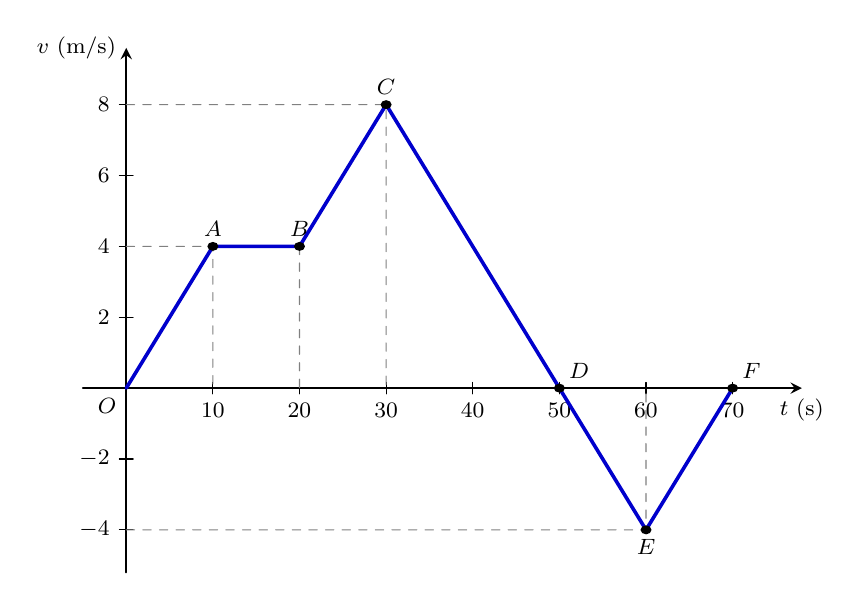
\begin{tikzpicture}[>=stealth, line join=round, line cap=round, font=\footnotesize, xscale=1.1, yscale=0.9]
	% Tọa độ các điểm
	\coordinate (O) at (0,0);
	\coordinate (A) at (1,2);
	\coordinate (B) at (2,2);
	\coordinate (C) at (3,4);
	\coordinate (D) at (5,0);
	\coordinate (E) at (6,-2);
	\coordinate (F) at (7,0);

	% Hệ trục tọa độ
	\draw[->, thick] (-0.5, 0) -- (7.8, 0) node[below] {$t\text{ (s)}$};
	\draw[->, thick] (0, -2.6) -- (0, 4.8) node[left] {$v\text{ (m/s)}$};
	\node[below left] at (0, 0) {$O$};

	% Vạch chia và nhãn trục hoành (t)
	\foreach \x/\t in {1/10, 2/20, 3/30, 4/40, 5/50, 6/60, 7/70} {
		\draw (\x, 0.08) -- (\x, -0.08);
		\node[below] at (\x, -0.08) {$\t$};
	}

	% Vạch chia và nhãn trục tung (v)
	\foreach \y/\v in {-2/-4, -1/-2, 1/2, 2/4, 3/6, 4/8} {
		\draw (0.08, \y) -- (-0.08, \y);
		\node[left] at (-0.08, \y) {$\v$};
	}

	% Đường biểu diễn nét đậm
	\draw[line width=1.3pt, blue!80!black] (O) -- (A) -- (B) -- (C) -- (D) -- (E) -- (F);

	% Đường dóng nét đứt
	\draw[dashed, gray] (0, 2) -- (A) -- (1, 0);
	\draw[dashed, gray] (B) -- (2, 0);
	\draw[dashed, gray] (0, 4) -- (C) -- (3, 0);
	\draw[dashed, gray] (0, -2) -- (E) -- (6, 0);

	% Điểm và nhãn
	\foreach \p/\g in {A/above, B/above, C/above, D/above right, E/below, F/above right} {
		\fill[black] (\p) circle (1.8pt);
		\node[\g] at (\p) {$\p$};
	}
\end{tikzpicture}
\end{document}
